\documentclass{beamer}
\usetheme{metropolis}
\metroset{block=fill}

\usepackage[T1]{fontenc}
\usepackage{microtype}

\usepackage{soul}
\usepackage{appendixnumberbeamer}

\usepackage{tikz}
\tikzset{every picture/.append style={font=\ttfamily}}
\usepackage{forest}
\forestset{
    default preamble={
        font=\ttfamily,
    }
}

% FiraFonts
\usepackage[sfdefault,scale=0.87]{FiraSans}
\usepackage[scale=0.87]{FiraMono}
% Use thinner fonts
\makeatletter
\def\bfseries@sf{medium}
\def\mdseries@sf{l}
\makeatother

\usepackage{listings}

\lstdefinelanguage{fsharp}{
    morekeywords = {type, member, new, let, let!, return, for, yield}
}

\lstdefinelanguage{scala}{
    morecomment=[l]{//},
    morekeywords = {sealed, type, override, val, var, trait, case, class, def, extension, extends, with, if, then, else, while, do, for, yield, inline, enum, object}
}

\lstset{
    keepspaces=true,
    breaklines=true,
    breakatwhitespace=true,
    columns=fixed,
    escapeinside=``,
    frame=tb,
    basicstyle=\small\ttfamily,
    commentstyle=\itshape,
    keywordstyle=\bfseries,
    language=scala
}

\newcommand{\scalasnippet}[1]{\lstinline[language=scala]{#1}}
\newcommand{\fssnippet}[1]{\lstinline[language=fsharp]{#1}}


\newcommand{\translation}[2][0.5]{%
    \begin{minipage}[t]{#1\textwidth - 0.05\textwidth}%
        \lstinputlisting[language=scala,frame=t]{#2/left.scala}%
    \end{minipage}%
    \hfill{}$\longmapsto$\hfill{}%
    \begin{minipage}[t]{0.95\textwidth - #1\textwidth}%
        \lstinputlisting[language=scala,frame=t]{#2/right.scala}%
    \end{minipage}
    \rule{\textwidth}{0.4pt}
}

\newcommand{\equivalent}[1]{%
    $\equiv$\hfill{}%
    \begin{minipage}[t]{0.95\textwidth}%
        \lstinputlisting[language=scala,frame=t]{#1/bot.scala}%
    \end{minipage}
    \rule{\textwidth}{0.4pt}
}

\author{Noé De Santo}
\title{Computation expressions for Scala 3}
\subtitle{From AST builders to computation expressions}
\date{17 June 2022}

\begin{document}

    \maketitle

    \section{Motivating example}

    \begin{frame}{Simple planes...}
        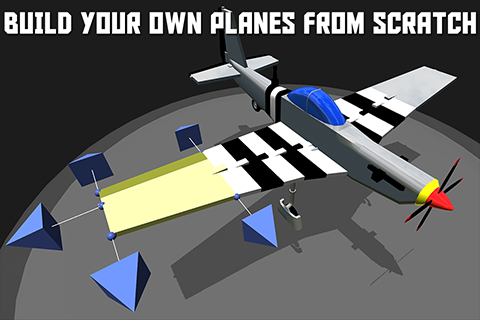
\includegraphics[width=\textwidth]{figs/simple_planes.png}
    \end{frame}

    \begin{frame}{...are not simple to program}
        \lstinputlisting[basicstyle=\tiny\ttfamily]{code/funky/xml_sample.xml}
        \vspace{2em}
        \pause
        \lstinputlisting{code/funky/scala_sample.scala}
    \end{frame}

    \begin{frame}{What are we doing?}
        Goals:
        \begin{itemize}
            \item Design and implement a library allowing to ``program'' ASTs inside of Scala;
            \item Generalize it as much as possible.
        \end{itemize}

        \pause
        Potential use cases:
        \begin{itemize}
            \item ``Little languages'';
            \item Configuration generation (yaml, kubernetes, \ldots{});
            \item Programmatic drawing (dot, miro, tikz, \ldots{}).
        \end{itemize}
        % Could be used for more little languages
        % configurations (yaml, kubernetes)/devops
        % miro (diagrams)
    \end{frame}

    \section{Foreword:\\Today's toy example}

    \begin{frame}{Meet Rob}
        We will work with an imaginary programmable robot, Rob.
        \begin{itemize}
            \item Lives on a 2D grid;
            \item Can move forward, rotate on itself;
            \item Know things about itself (position, orientation);
            \item Typical features (variables, if-then-else, statement sequencing, \ldots{}).
        \end{itemize}

        AST represented using type \scalasnippet{Tree[_]}.

        \pause
        To make it easier to use, we will also assume a
        \scalasnippet{Conversion[Int, Tree[Int]]}
    \end{frame}

    \begin{frame}{A Rob example}
        \lstinputlisting{code/rob_example.scala}

        \scalebox{0.8}{%
            \begin{forest}
                [;
                    [Initialize [x] [0]]
                    [;
                        [While [!{=}{=} [robOrientation] [Orientation.N]] [robRotateLeft]]
                        [; [robAdvance] [robAdvance]]
                    ]
                ]
            \end{forest}
        }
    \end{frame}

    \section{Implementation\\\footnotesize{(And why not all of this is a good idea)}}

    \begin{frame}{Metaprogramming}
        Key idea:
        \begin{itemize}
            \item We can leverage Scala's metaprogramming to replace some constructs;
        \end{itemize}
        \translation{code/rewriting}
        \begin{itemize}
            \item<2-> Here, we are basically overloading the (implicit) \lstinline{;} operator;
            \item<2-> The same can be done for other constructs (e.g. assignation \lstinline{=}).
        \end{itemize}
    \end{frame}

    \begin{frame}{Variables translation}
        This requires to correctly dissociate between the Scala-level variable, and the user-language-level one:

        \translation{code/variable}

        \pause
        Which, after further transformation and Scala execution, yields:
        
        \equivalent{code/variable}
    \end{frame}

    \begin{frame}{Typing issues}
        \only<1>{
            We might have some typing issues:
            \lstinputlisting{code/broken_types.scala}
        }
        \only<2->{
            We \st{might} have \st{some} \textbf{many} typing issues:
            \lstinputlisting{code/broken_types_hg.scala}
            (Note that, after transformation, the code is well-typed, and has type \lstinline{Tree[Unit]})
        }
        \only<3->{
            Solutions:
            \begin{enumerate}
                \item Do it differently;
                \item Trick the type system into accepting this.
            \end{enumerate}
        }
    \end{frame}

    \begin{frame}{hippity hoppity accept my code}
        We can (ab-)use implicit conversions. We would need:
        \begin{center}
            \begin{tabular}{lll}
                \lstinline{Tree[T]} & $\longmapsto$ & \lstinline{Variable[T]} \\ % Var assignation
                \lstinline{Tree[Boolean]} & $\longmapsto$ & \lstinline{Boolean} \\ % if-then-else
                \lstinline{Unit} & $\longmapsto$ & \lstinline{Tree[Unit]} % assignation typing
            \end{tabular}
        \end{center}

        \pause
        Issues:
        \begin{itemize}
            \item Can be inserted in unexpected (and unwanted) places;
            \item Highly contextual;
            \item Technically, do not convert anything: they will get erased.
        \end{itemize}
    \end{frame}

    \begin{frame}{Think different}
        \begin{enumerate}
            \item Use DSL elements to replace some constructs:\begin{itemize}
                \item Step away from Scala notations;
                \item No typing-trickery.
            \end{itemize}
            \item Use an operator to signify user-level variables.
        \end{enumerate}

        \only<2>{
            \begin{center}
                \begin{tabular}{lll}
                    \lstinline{val x = value} & $\longmapsto$ & \lstinline{val x = ! (value)} \\ % Var assignation
                    \lstinline{if cond then thenn else elze} & $\longmapsto$ & \lstinline{If(cond)\{ thenn \}\{ elze \}} \\ % if-then-else
                    \lstinline{variable = value} & $\longmapsto$ & \lstinline{variable =! value} % assignation typing
                \end{tabular}
            \end{center}
        }
        \only<3>{
            \lstinputlisting{code/fixed_types.scala}
        }
    \end{frame}

    \section{Generalization:\\toward computation expressions}

    \begin{frame}{More than Rob}
        The previous examples were tied to our robot. Solution:
        \begin{itemize}
            \item Let the user define a \lstinline{myBuilder};
            \item<2-> Call the methods of the builder.
        \end{itemize}
        \only<1>{
            \lstinputlisting{code/builder.scala}
        }
        \only<2>{
            \translation[0.48]{code/rewriting_builder}
        }

    \end{frame}

    \begin{frame}{Computation expresions: Qu'es aquò?}
        To keep it short and simple:
        \begin{itemize}
            \item Feature of F\# (functional language; .NET based);
            \item Some keywords ``do nothing'' (e.g. \fssnippet{let!});
            \item A function can be implemented to give meaning to them.
        \end{itemize}
    \end{frame}

    \begin{frame}{Call it maybe}
        \lstinputlisting[language=fsharp]{code/maybe.fs}
    \end{frame}

    \begin{frame}{The anatomy of \fssnippet{Bind}}
        \fssnippet{Bind}/\fssnippet{let!} takes two arguments: the value being bound, and the ``follow''.

        \begin{minipage}[t]{0.45\textwidth}%
            \lstinputlisting[language=fsharp,frame=t]{code/bind_anat/left.fs}%
        \end{minipage}%
        \hfill{}$\longmapsto$\hfill{}%
        \begin{minipage}[t]{0.45\textwidth}%
            \lstinputlisting[language=fsharp,frame=t]{code/bind_anat/right.fs}%
        \end{minipage}
        \rule{\textwidth}{0.4pt}

        \pause 
        Reminds me a lot of:
        \begin{block}{Encoding let}
            \[\textup{let } x = t_1;\ t_2 \qquad \equiv \qquad (\lambda x.\ t_2)(t_1)\]
        \end{block}
    \end{frame}

    \begin{frame}{AST builders as computation expressions}

        In the context of AST builders,
        we can use this to get back our original transformation.

        \only<1-2>{
            \translation[0.3]{code/variable_ce}
            \pause 
            \equivalent{code/variable_ce}
        }

        \only<3>{
            \lstinputlisting{code/ast_bind.scala}
        }
    \end{frame}

    \section{Wrapping up}

    \begin{frame}{What exactly was done?}
        \begin{itemize}
            \item Some (restricted) form of computation expressions were implemented;
            \item AST builders were defined as some particular kind of computation expressions;
            \item DSL was privileged over implicit conversions.
        \end{itemize}
    \end{frame}

    \begin{frame}{Does this generalize?}
        \begin{itemize}
            \item Computation expressions are (by design) general, yet restricted in our case;
            \item AST builders seem general enough in our examples.
        \end{itemize}
    \end{frame}

    \appendix

    \begin{frame}{3-sort}
        \lstinputlisting[basicstyle=\tiny\ttfamily,frame=]{code/examples/3-sort.scala}
    \end{frame}

    \begin{frame}{Krakabloa race}
        \lstinputlisting[basicstyle=\tiny\ttfamily,frame=]{code/examples/KrakabloaRace.scala}
    \end{frame}

    \begin{frame}[standout]
        The End (?)
    \end{frame}

    \begin{frame}{References}
        \begin{itemize}
            \item The result: \url{https://github.com/Ef55/scala-expression-processor}
            \item Computation expressions: \url{https://docs.microsoft.com/en-us/dotnet/fsharp/language-reference/computation-expressions}
            \item CE usage: \url{https://link.springer.com/chapter/10.1007/978-3-319-04132-2_3}
        \end{itemize}
    \end{frame}

    \begin{frame}{What do you mean ``restricted''?}
        \begin{itemize}
            \item F\#'s CE do not enforce one particular (type-)signature;
            \item We fixed one for practical purposes.
        \end{itemize}
        \scalasnippet{(Computation[T], B[T] => Computation[S]) => Computation[S]}
        where \scalasnippet{B} is a type function.
    \end{frame}

    \begin{frame}{Why this weird signature in particular?}
        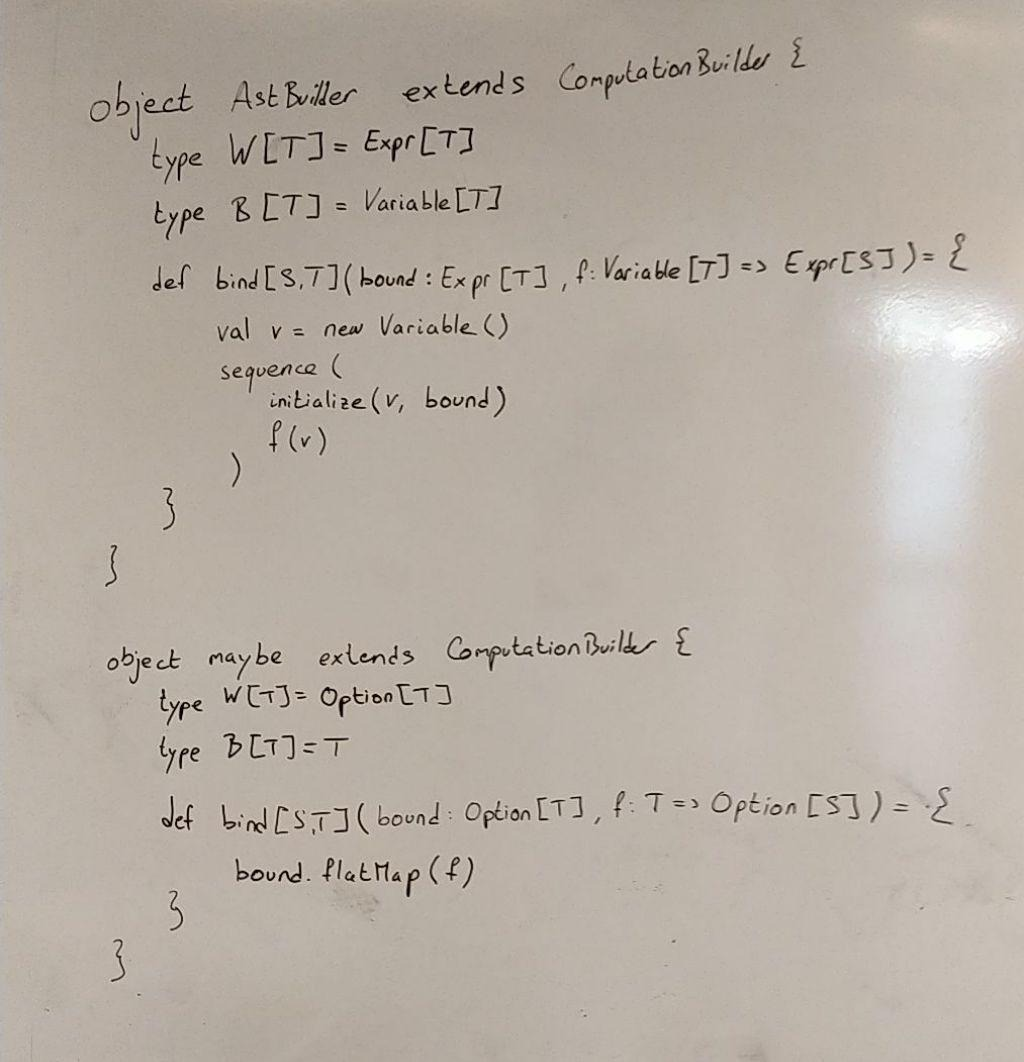
\includegraphics[width=0.7\textwidth]{figs/reasoning.jpeg}
    \end{frame}

    \begin{frame}{What if ``!'' is ambiguous?}
        Our ``binding'' \scalasnippet{!} is defined on \scalasnippet{Tree}/\scalasnippet{Computation}:

        \translation{code/implicit/int}

        \translation{code/implicit/bool}

        If \scalasnippet{!} is defined on the type aliased by \scalasnippet{Tree}/\scalasnippet{Computation}, there is indeed an issue.
    \end{frame}

    \begin{frame}{Why so parametric?}
        \url{https://github.com/lampepfl/dotty/issues/15176}

        tldr; bug in type equality in presence of aliasing/path-dependent types.
    \end{frame}

\end{document}